% falar da modelagem

Assim como citado na sessão anterior, a árvore de sufixos foi criada com base
numa \textit{trie compacta}.
Isso significa que o objetivo dessa estrutura é tentar minimizar o custo de
espaço.
Para isso, cada nó, ao invés de armazenar \textit{sub strings} provenientes
do texto original, armazena uma tupla com um valor \texttt{inicio} e
\texttt{fim}.
Essa tupla representa os índices de determinada substring contida no texto
fazendo com que a rearmazenagem do texto não seja necessária e redundante,
por consequência.
Além disso, é valido ressaltar que o grafo foi implementado através de uma lista
de adjacências.
Sendo assim, as arestas da árvore são representadas por uma lista contendo todos
os nós filhos de um nó pai, não existindo uma estrutura de dados criada
especificamente para descrever as aresta, uma vez que trata-se apenas de um
link entre dois nós, nessa implementação.
Conclui-se portanto, que todas as informações são armazenadas nos nós.

Um outro fator que mere relevância é a adição de um atributo \textit{booleano}
na estrutura \textbf{nó}.
O objetivo dessa informação é apenas indicar se determinado nó da árvore pode
ser identificado como um um sufixo do texto.
Em algumas notações de implementação, costuma-se utilizar o caractere cifrão
('\$') para tal representação.
Porém, apenas por uma questão de generalização, optou-se por não adicionar um
caractere especial ao texto a fim de garantir que tal solução funcione mesmo
para os casos em que esse símbolo faça parte do alfabeto do texto.
Dessa maneira, a estrutura do tipo \textbf{Nó} é denotada por:

\begin{figure}[h]
	\begin{center}
		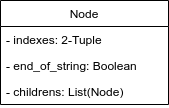
\includegraphics[scale=0.75]{Figuras/node.png}
	\end{center}
	\caption{\label{fig:node} Estrutura de um nó.}
\end{figure}

A partir do modelo de nó da Figura \ref{fig:node} a árvore de sufixos é
construída.
A classe que controla árvore tem apenas dois atributos, um deles é do tipo
\textbf{Nó} e representa a raíz da árvore.
Já o outro atributo é o texto o qual a árvore será montada.
Portanto os nós internos da árvore são obtidos apenas no caminhamento recursivo
entre os nós que estão "abaixo" da raiz.
Em resumo, com excessão da raíz da árvore, nenhum dos demais nós é um atributo
próprio da classe \textbf{SufixTree}.
Isso faz com que o princípio do encapsulamento seja garantido.

\begin{figure}[h]
	\begin{center}
		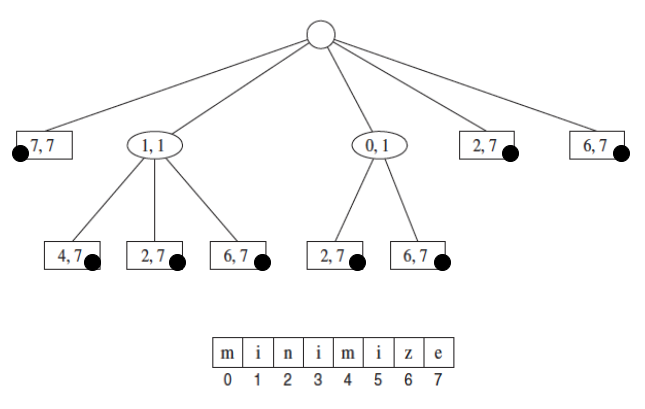
\includegraphics[scale=0.5]{Figuras/compact-trie.png}
	\end{center}
    \caption{\label{fig:compact-trie} Exemplo de uma árvore de sufixos para a palavra "minimize".}
\end{figure}


A Figura \ref{fig:compact-trie} representa como se daria uma árvore a partir da
solução empregada nesse trabalho.
Relacionando as Figuras \ref{fig:node} e \ref{fig:compact-trie} temos que o par
de número inteiros contidos no interior de cada nó se trata do atributo
\texttt{indexes}, o circulo preto indica que a marcação de fim de string é
verdadeiro.
Porém, a lista de adjacência é expressada para cada aresta que parte de um nó em
direção a um nó mais profundo.
Pode-se tomar como exemplo o nó \texttt{(0, 1)} que tem \texttt{(2, 7)} e
\texttt{(6, 7)} em sua lista de adjacências.
